\section{Numerical Experiments for the Stokes Equations}
\label{sec:StokesNumericalResults}
To illustrate the theoretical results, we perform three numerical
experiments.  In the first two we use boundary conditions and forcing
function corresponding to a manufactured solution; first showing
optimal convergence using the graph norm arising from the analysis as
the test space norm, then showing sub-optimal convergence when a naive
norm is selected instead.  Finally, we examine the classic lid-driven
cavity flow problem.

We implemented the experiments described below using \emph{Camellia}, a toolbox for DPG developed by Roberts starting at Sandia in summer 2011, in collaboration with Denis Ridzal and Pavel Bochev \cite{RobertsEtAl11}.  Camellia supports 2D meshes of triangles and quads of variable polynomial order, provides mechanisms for easy specification of DPG variational forms, supports $h$- and $p$- refinements, and supports distributed computation of the stiffness matrix, among other features.

Recall that the pressure $p$ in the Stokes problem is only determined up to a constant.  Following a method described by Bochev and Lehoucq \cite{BochevLehoucq}, we add a constraint on the pressure that enforces
\[
\int_{\Omega} p = 0,
\]
thereby determining the solution uniquely.  This constraint is also satisfied by the manufactured solution used in our experiments.

Before turning to the experiments themselves, we briefly note the expected convergence properties and give a few implementation details.  When implementing DPG, we have several choices: what polynomial orders to use for the approximation of fields, traces, and fluxes; how to approximate the optimal test functions, and what norm to use on the test space.  We discuss each of these in turn.

\subsection{Convergence and orders of polynomial approximation}
For a DPG solution $(u_{h},\widehat{u}_{h})$ and exact solution $(u,\widehat{u})$, the analysis in Appendix \ref{sec:StokesAnalysis} gives us
\begin{align}\label{NVR:eqn:gammaBound}
\left(\norm{u-u_{h}}^{2} + \norm{\widehat{u}-\widehat{u}_{h}}_{\hat{H}_A(\Gamma_{h})}^{2}\right)^{1/2} \leq \frac{M}{\gamma_{DPG}} \inf_{(w_{h},\widehat{w}_{h})}\left(\norm{u-w_{h}}^{2} + \norm{\widehat{u}-\widehat{w}_{h}}_{\hat{H}_A(\Gamma_{h})}^{2}  \right)^{1/2},
\end{align}
where $M=O(1)$ and $\gamma_{DPG}=O(\gamma)$ (and for the Stokes problem, $\gamma=O(1)$), the salient point for convergence being that these are mesh-independent constants: for the graph norm presented in the analysis, the method is automatically stable.\footnote{As will be seen in what follows, if we use the naive test norm instead, we do \emph{not} get the optimal convergence rates in the pressure.  We hypothesize that if we performed a similar analysis for the naive norm, $\gamma$ would not be mesh-independent.}

Assuming $u$ is sufficiently smooth, for a discrete $L^2$ space comprised of polynomials of order $k$, we expect best $h$-convergence rates of $k+1$; that is, we have
\begin{align}
\inf_{w_{h} \in U_{h}} \norm{u-w_{h}} \leq C_{1} h^{k+1}.\label{NVR:eqn:hBound}
\end{align}
for some mesh-independent constant $C_{1}$.  It can be shown that, for traces $\widehat{w}_{h}$ whose $H^{-1/2}(\Gamma_{h})$ and $H^{1/2}(\Gamma_{h})$ components are approximated by polynomials of orders $k$ and $k+1$, respectively,
\[
\inf_{\widehat{w}_{h} \in \hat{H}_A(\Gamma_{h})} \norm{\widehat{u}-\widehat{w}_{h}}_{\hat{H}_A(\Gamma_{h})} \leq C_{2} h^{k+1}
\]
for some mesh-independent constant $C_{2}$.  For details and further references, see \cite[pp. 7-8]{DPG6}. Combining this with equations (\ref{NVR:eqn:gammaBound}) and (\ref{NVR:eqn:hBound}), we then have the bound
\[
\norm{u-u_{h}} \leq C h^{k+1}
\]
for $C = \min(C_{1}, C_{2})$.
Assuming negligible error in computing the optimal test functions, for these choices of polynomial order, we expect DPG solutions to converge in $h$ at the optimal rate of $k+1$ for all $L^{2}$ variables.

We can also motivate the choice of polynomial orders for the trial space intuitively from the exact sequence.  If we define $k$ as the polynomial order of approximation of field variables, because these belong to $L^{2}$, it is natural to choose $k+1$ as the $H^{1}$ order.  The traces of $H^{1}$ functions ($\widehat{u}_{1}$ and $\widehat{u}_{2}$) belong to $H^{1/2}$, a stronger space than $L^{2}$, so that $k+1$ is a natural order of approximation for these.  The traces of \NVRHdiv  functions $\left(\widehat{{\sigma_{11} - p \choose \sigma_{12}} \cdot \vect{n}}\right.$ and $\left.\widehat{{\sigma_{21}  \choose \sigma_{22} - p} \cdot \vect{n}}\right)$ belong to $H^{-1/2}$, a weaker space than $L^{2}$, so that $k$ is a natural order of approximation for these.

The exact optimal test functions will not in general be polynomials; we approximate them by using an ``enriched'' space of Lagrange and Raviart-Thomas elements approximating $H^{1}(\Omega_{h})$ and $\vect{H}(\text{\rm div},\Omega_{h})$ components of the test space.  In practice, we experiment with various levels of enrichment, and take the minimum enrichment that yields results nearly as good as higher levels of enrichment.  In the present work, we used 1 as the enrichment order; that is, $k_{\rm test} = k+2$.  As will be seen below, with this, we come extremely close to matching the best approximation error, so that there is no benefit to enriching the test space further.\footnote{For an analysis of the effect of the test space enrichment on rates of convergence in the Laplace problem and linear elasticity, see Gopalakrishnan and Qiu \cite{GopalakrishnanQiu11}.}

Note also that we have made no assumptions about the choice of basis functions.  The present work uses $H^{1}$- and \NVRHdiv-conforming nodal bases provided by the Intrepid package in Trilinos \cite{Trilinos}.

\subsection{Test space norm}
The choice of test norm arising from the above analysis is the (adjoint) graph norm:
\begin{align*}
\norm{(\NVRtensor{\tau},\vect{v}, q)}_{\rm graph}^{2} = \norm{\NVRdiv \NVRtensor{\tau} - \NVRgrad q}^{2} + \norm{\NVRdiv \vect{v}}^{2} + \norm{ \NVRtensor{\tau} + \NVRgrad{\vect{v}}}^{2} + \norm{\NVRtensor{\tau}}^{2} + \norm{\vect{v}}^{2} + \norm{q}^{2}
\end{align*}

We use this norm in our first experiment, and get the optimal convergence rates for the field variables.  In our second experiment, we consider another choice of test norm, which we refer to as the \emph{naive} test space norm:
\begin{align*}
\norm{(\NVRtensor{\tau},\vect{v}, q)}_{\rm naive}^{2} = \norm{\NVRtensor{\tau}}^{2} + \norm{\NVRdiv \NVRtensor{\tau}}^{2} + \norm{\vect{v}}^{2} + \norm{\NVRgrad \vect{v}}^{2} + \norm{q}^{2} + \norm{\NVRgrad q}^{2}.
\end{align*}
Note that this is a \emph{stronger} space than the one generated by the graph norm; that is, if we define
\begin{align*}
\V_{\rm graph} &= \{ (\NVRtensor{\tau},\vect{v}, q) : \norm{(\NVRtensor{\tau},\vect{v}, q)}_{\rm graph} < \infty \}, \text{and} \\
\V_{\rm naive} &= \{ (\NVRtensor{\tau},\vect{v}, q) : \norm{(\NVRtensor{\tau},\vect{v}, q)}_{\rm naive} < \infty \},
\end{align*}
then $V_{\rm naive} \subset V_{\rm graph}$.  Specifically, $V_{\rm graph}$ only requires $\NVRdiv \NVRtensor{\tau} - \NVRgrad q \in \vect{L}^{2}$, while $V_{\rm naive}$ requires $\NVRdiv \NVRtensor{\tau} \in \vect{L}^{2}$ \emph{and} $\NVRgrad q \in \vect{L}^{2}$.

\subsection{Manufactured Solution Experiment with Graph Test Space Norm}
To test the method, we use a manufactured solution following Cockburn et al. \cite{CockburnKanschatSchotzauSchwab03}
\begin{align*}
u_{1} &=  -e^{x} ( y \cos y + \sin y )\\
u_{2} &=  e^{x}  y \sin y\\
p &= 2 \mu e^{x} \sin y
\end{align*}
on domain $\Omega = (-1,1)^2$, taking $\mu=1$, with uniform quadrilateral meshes of increasing granularity, and examine convergence rates.  The $L^{2}$ norm of the exact solution for $u_{1}$ is 2.53; for $u_{2}$, 1.07; for $p$, 2.81.

Figures \ref{fig:graph_h} and \ref{fig:graph_p} show $h$- and $p$-convergence\footnote{In this context, by $p$ we mean polynomial refinements.  We mostly use $k$ for polynomial order, because $p$ is our pressure variable; but a few times in the following pages we will overload $p$ to mean polynomial order as well.} results using the graph norm in the test space, for uniform quadrilateral meshes varying from $k=1$ to 4 in polynomial order, and from $1 \times 1$ to $16 \times 16$ elements.  The dashed lines in the plots show the error of an $L^{2}$ projection of the exact solution (the theoretical best we could achieve)---the lines lie nearly on top of each other.  We not only observe optimal convergence rates, but almost exactly achieve the best approximation error!

\begin{figure}[h!b!p!]
\centering
\subfigure[$u_{1}$]{
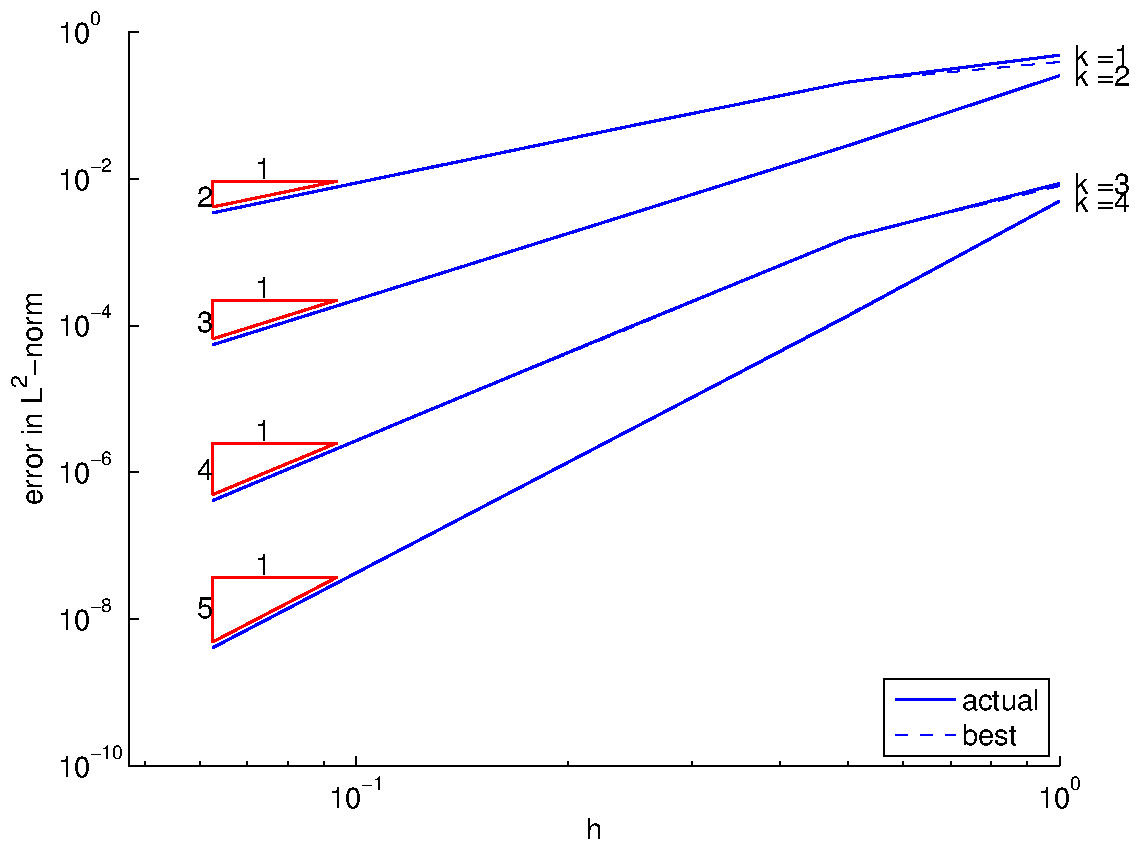
\includegraphics[scale=0.42]{./figures/u1_graph_h.pdf}
\label{fig:u1graph_h}
}
\subfigure[$u_{2}$]{
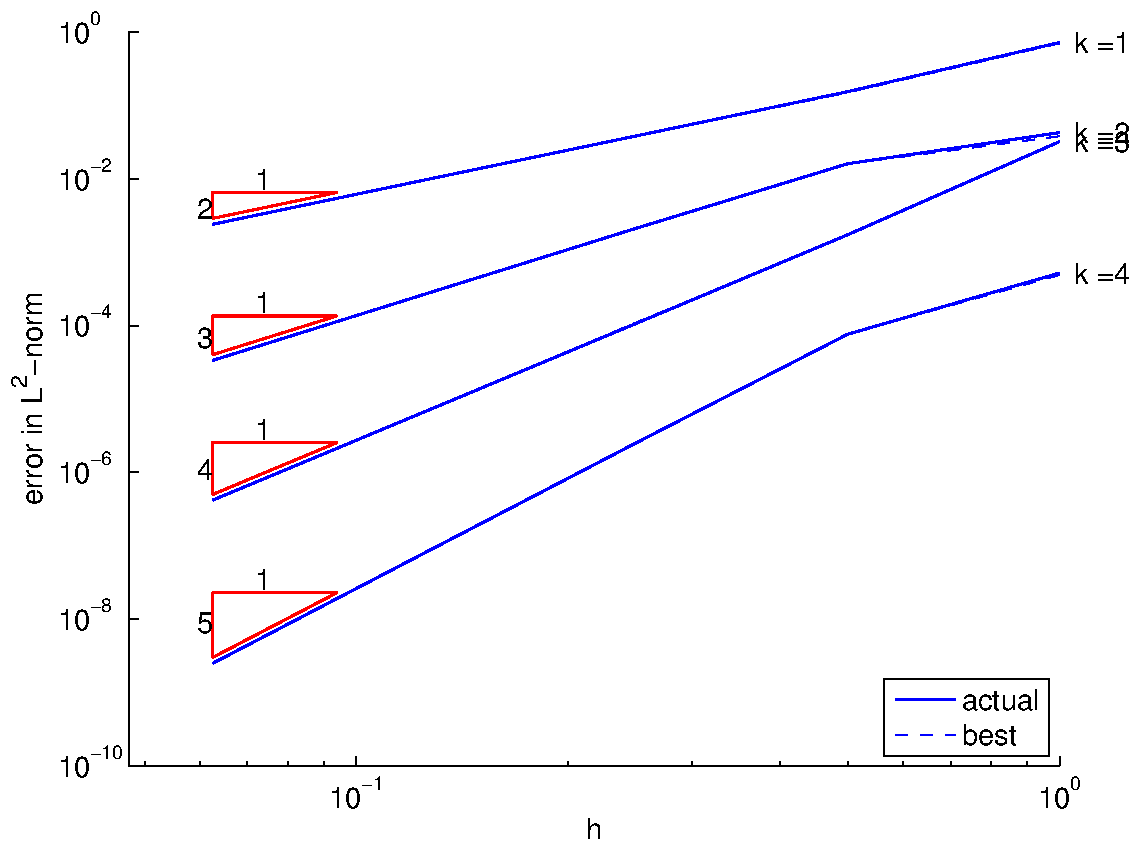
\includegraphics[scale=0.42]{./figures/u2_graph_h.pdf}
\label{fig:u2graph_h}
}
\subfigure[$p$]{
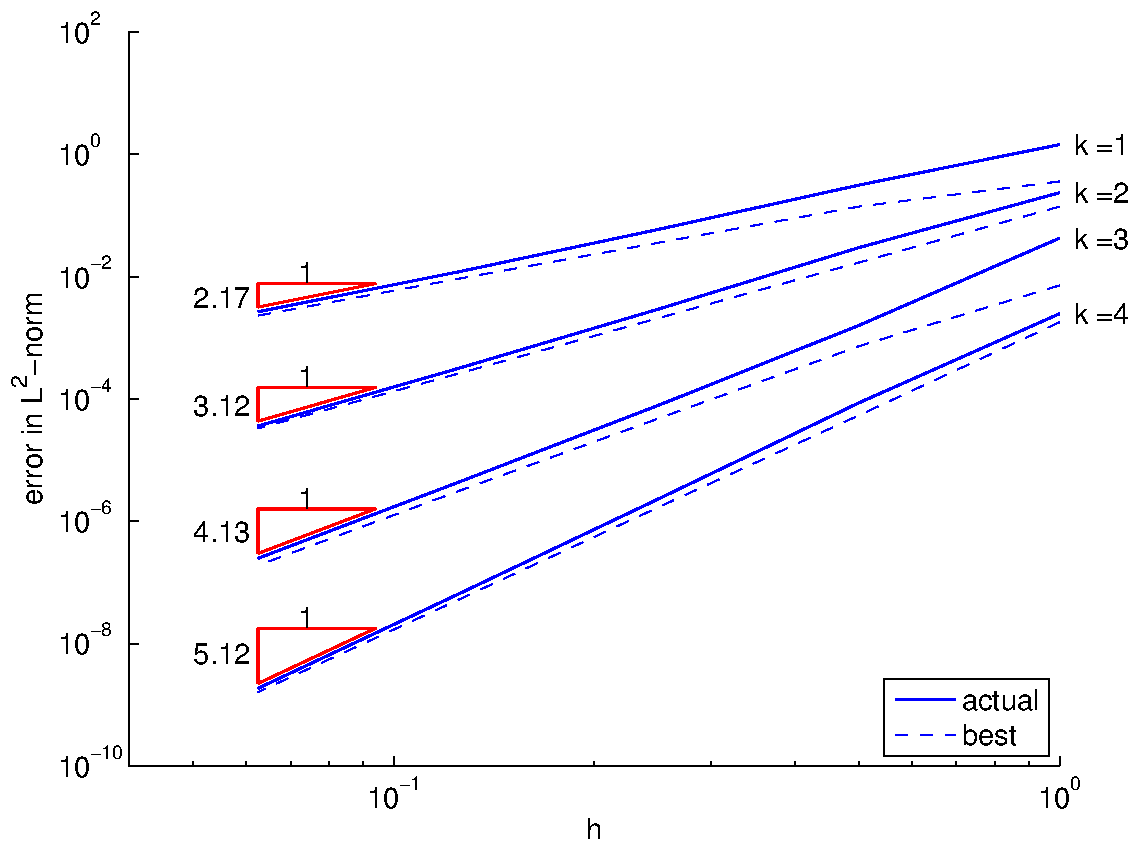
\includegraphics[scale=0.42]{./figures/pressure_graph_h.pdf}
\label{fig:pressuregraph_h}
}
\caption{$h$-convergence of $u_{1},u_{2}$ and $p$ when using the graph norm for the test space.  We observe optimal convergence rates, and nearly match the $L^{2}$-projection of the exact solution.
}
\label{fig:graph_h}
\end{figure}

\begin{figure}[h!b!p!]
\centering
\subfigure[$u_{1}$]{
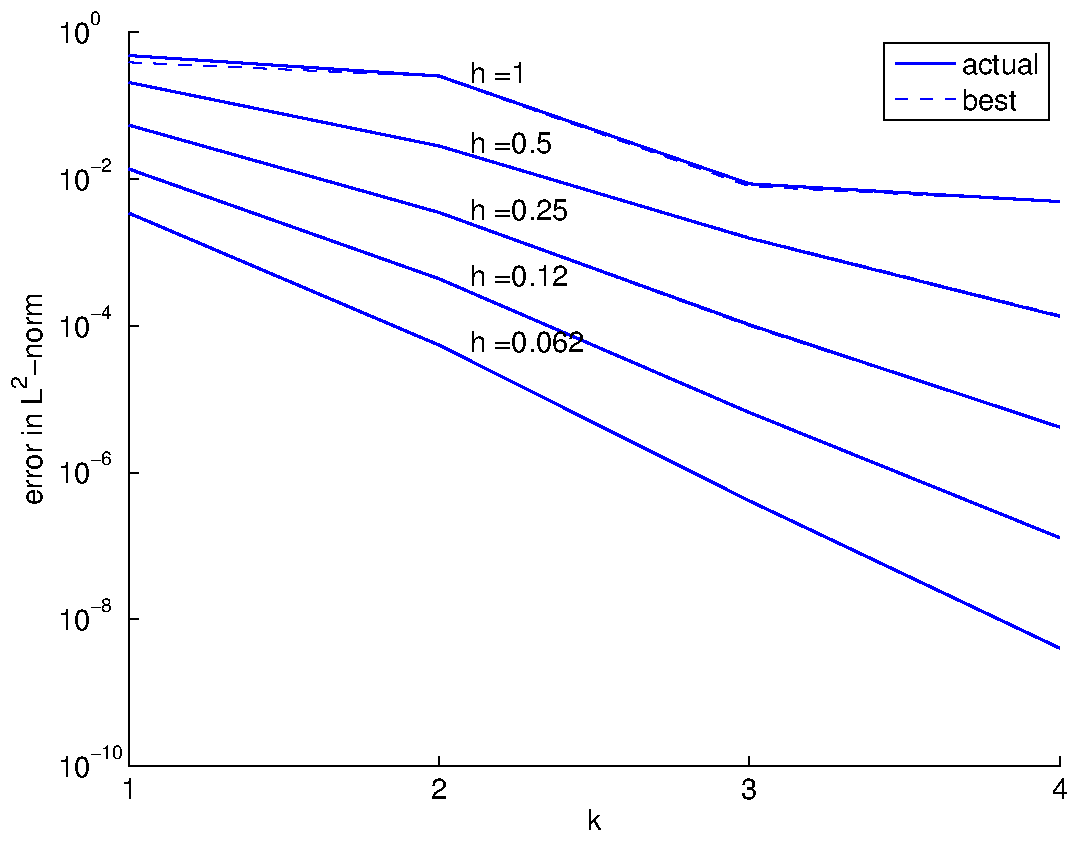
\includegraphics[scale=0.42]{./figures/u1_graph_p.pdf}
\label{fig:u1graph_p}
}
\subfigure[$u_{2}$]{
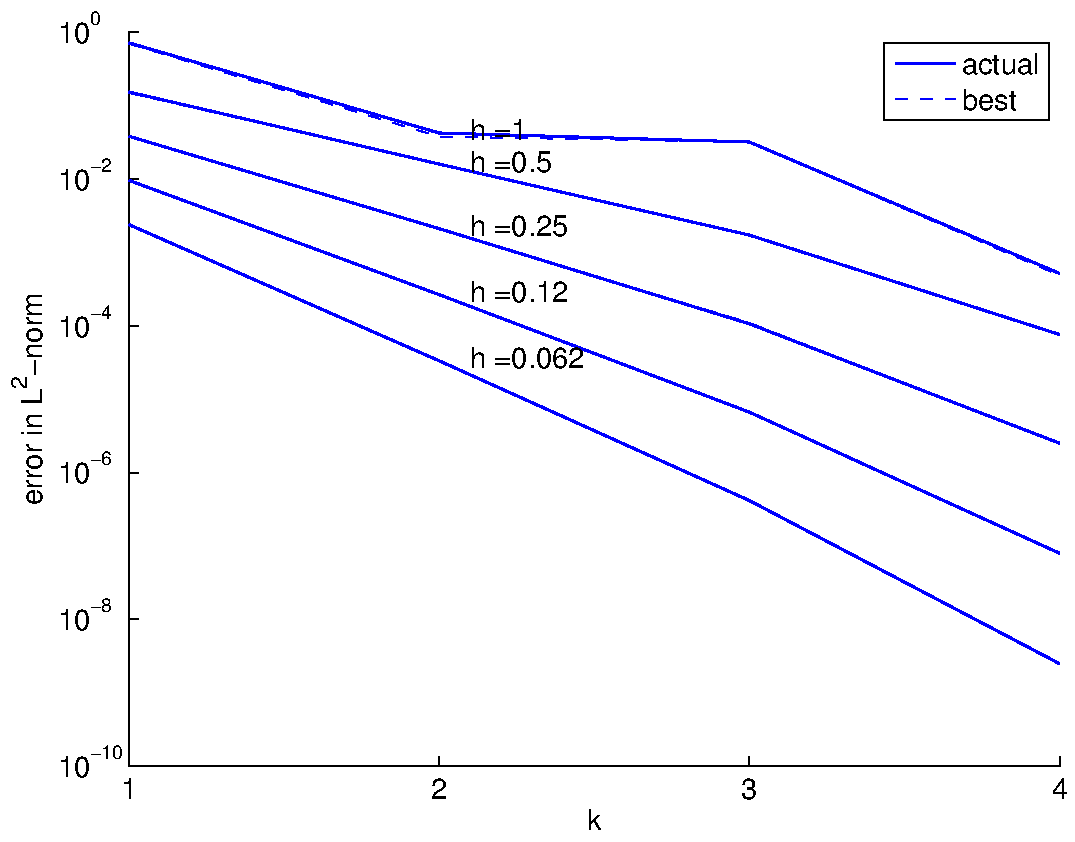
\includegraphics[scale=0.42]{./figures/u2_graph_p.pdf}
\label{fig:u2graph_p}
}
\subfigure[$p$]{
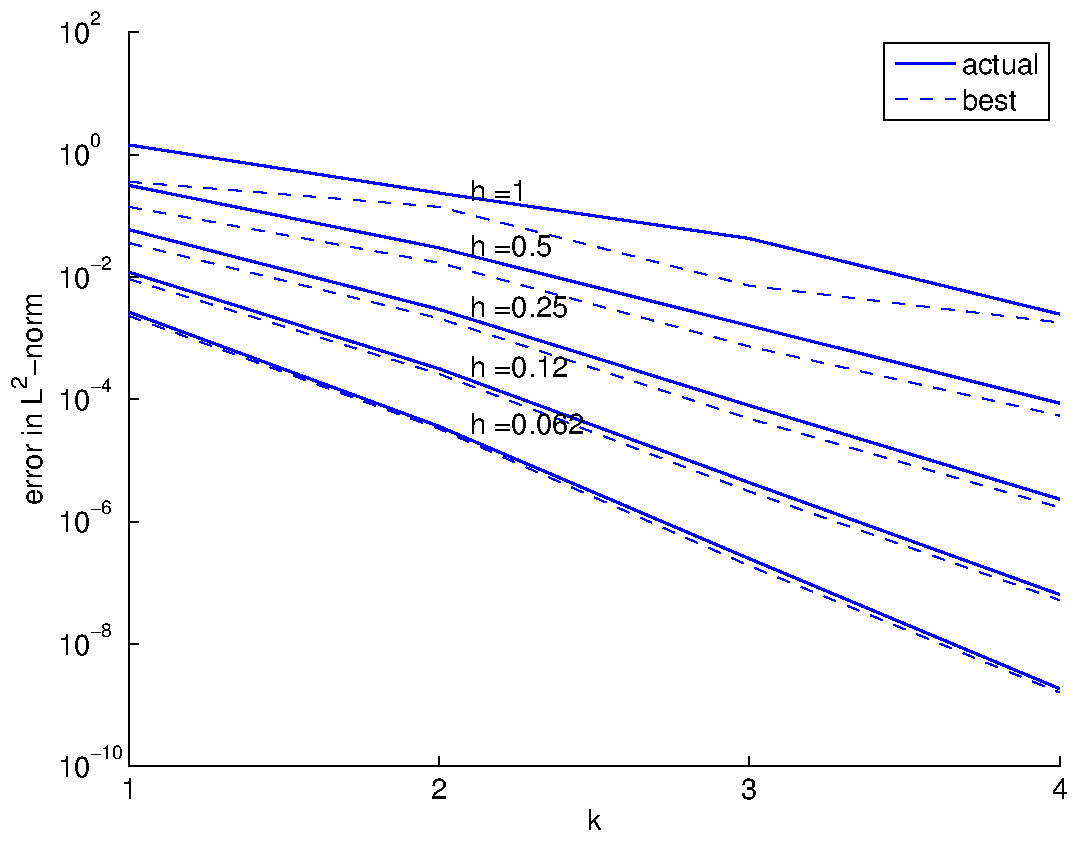
\includegraphics[scale=0.42]{./figures/pressure_graph_p.pdf}
\label{fig:pressuregraph_p}
}
\caption{p-convergence of $u_{1},u_{2}$ and $p$ when using the graph norm for the test space.  We observe exponential convergence for the finer meshes, and nearly match the $L^{2}$-projection of the exact solution.
}
\label{fig:graph_p}
\end{figure}

\subsection{Manufactured Solution Experiment with Naive Test Space Norm}
Our second manufactured solution experiment uses the naive norm on the test space.  This was the first norm we used when studying DPG formulations of Stokes \cite{RobertsetAl10}, before we had developed the analysis above, showing why the naive norm might not do as well as the graph norm does.

Figures \ref{fig:naive_h} and \ref{fig:naive_p} show $h$- and $p$-convergence results using the naive norm in the test space, for uniform quadrilateral meshes varying from $k=1$ to 4 in polynomial order, and from $1 \times 1$ to $16 \times 16$ elements; we have again plotted for comparison the error in the $L^{2}$ projection of the exact solution.  As with the graph norm, here we observe optimal convergence rates and almost exactly achieve the best approximation error in velocities $u_{1}$ and $u_{2}$, but in the pressure $p$ we are sub-optimal by up to two orders of magnitude.  

Why do we not see optimal convergence for the naive norm?  Recall that this is a stronger norm than the graph norm used in our analysis; thus the test functions that we seek---namely, the ones that will minimize the residual---may not reside within the continuous space represented by the naive norm.  By using the naive norm, we are searching for these test functions inside a smaller space, and we may not find them there.

\begin{figure}[h!b!p!]
\centering
\subfigure[$u_{1}$]{
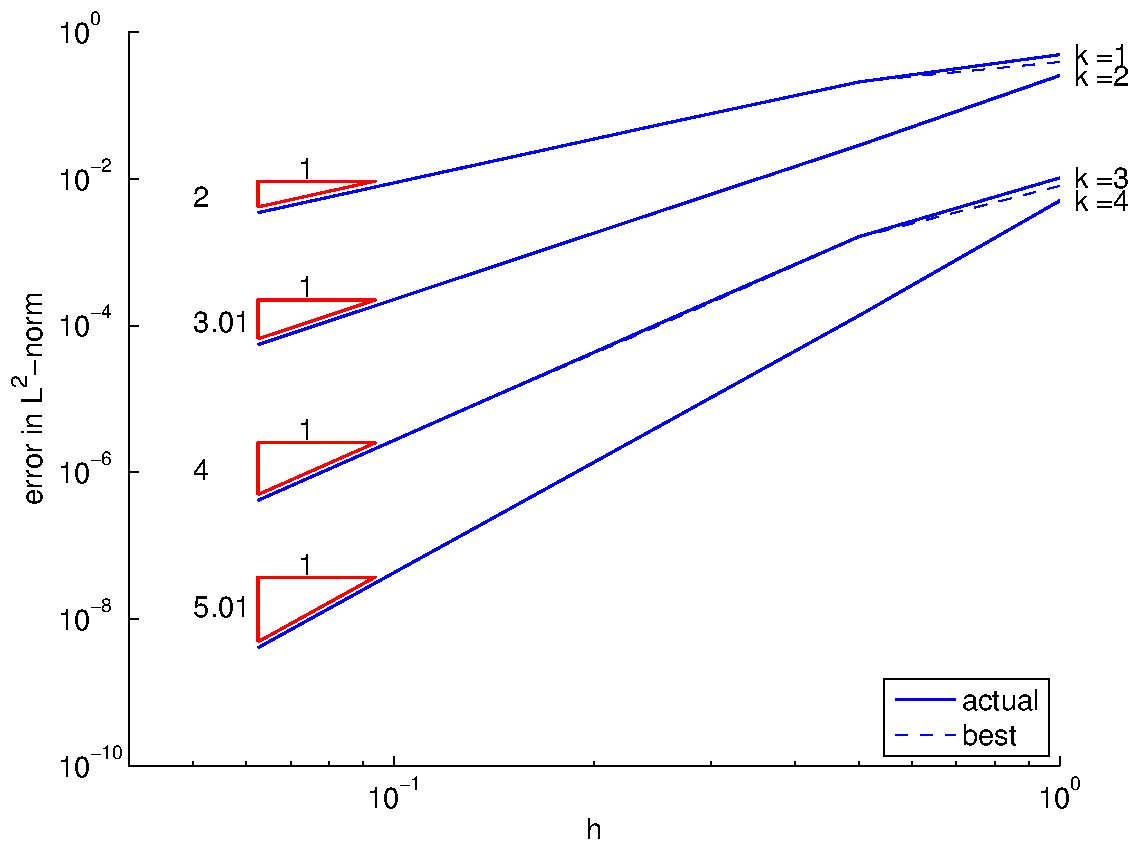
\includegraphics[scale=0.42]{./figures/u1_naive_h.pdf}
\label{fig:u1naive_h}
}
\subfigure[$u_{2}$]{
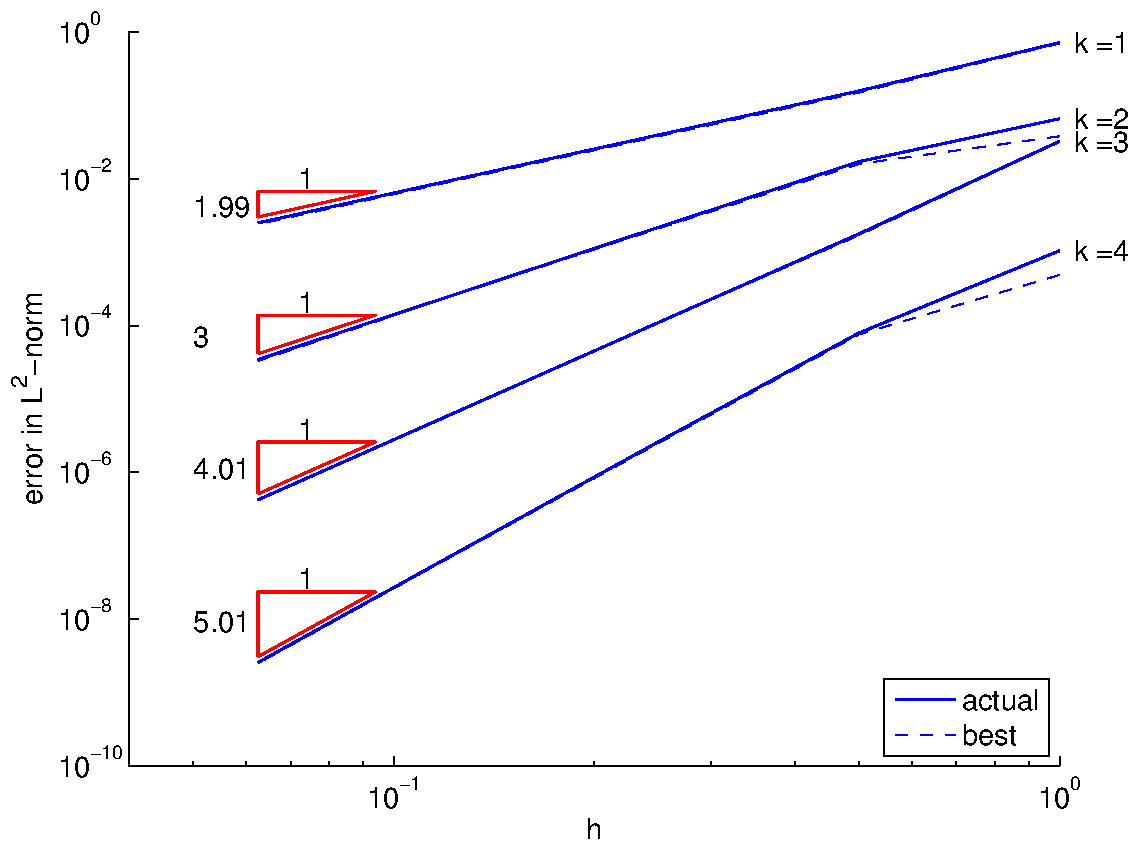
\includegraphics[scale=0.42]{./figures/u2_naive_h.pdf}
\label{fig:u2naive_h}
}
\subfigure[$p$]{
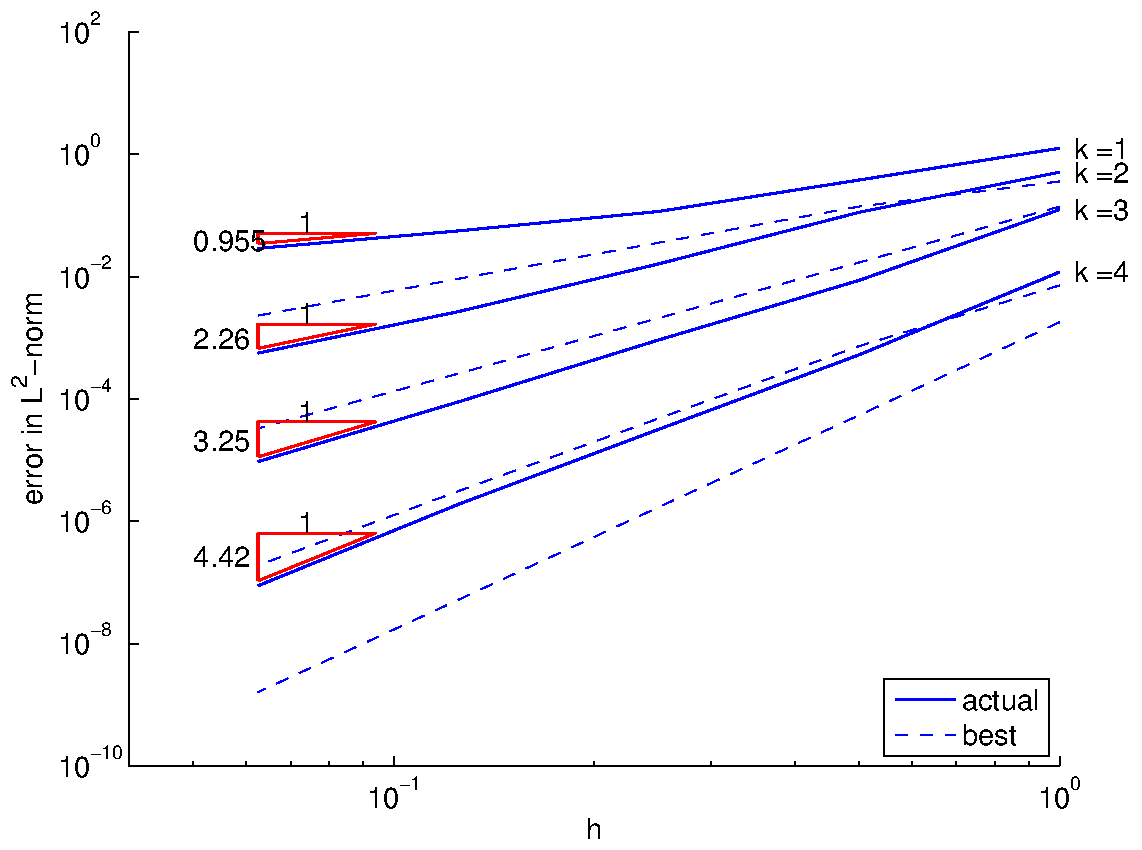
\includegraphics[scale=0.42]{./figures/pressure_naive_h.pdf}
\label{fig:pressurenaive_h}
}
\caption{$h$-convergence of $u_{1},u_{2}$ and $p$ when using the naive norm for the test space.  We observe optimal convergence rates (and nearly match the $L^{2}$-projection of the exact solution) for $u_{1}$ and $u_{2}$, but $p$ converges at suboptimal rates.
}
\label{fig:naive_h}
\end{figure}


\begin{figure}[h!b!p!]
\centering
\subfigure[$u_{1}$]{
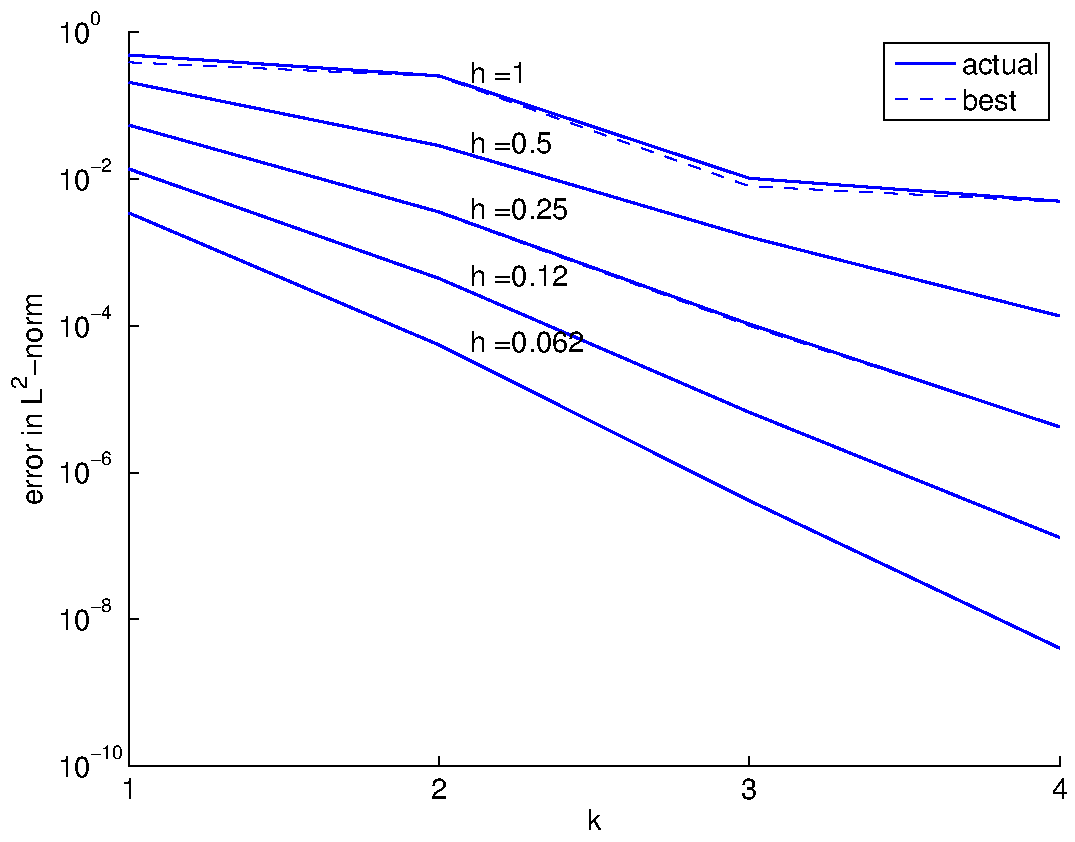
\includegraphics[scale=0.42]{./figures/u1_naive_p.pdf}
\label{fig:u1naive_p}
}
\subfigure[$u_{2}$]{
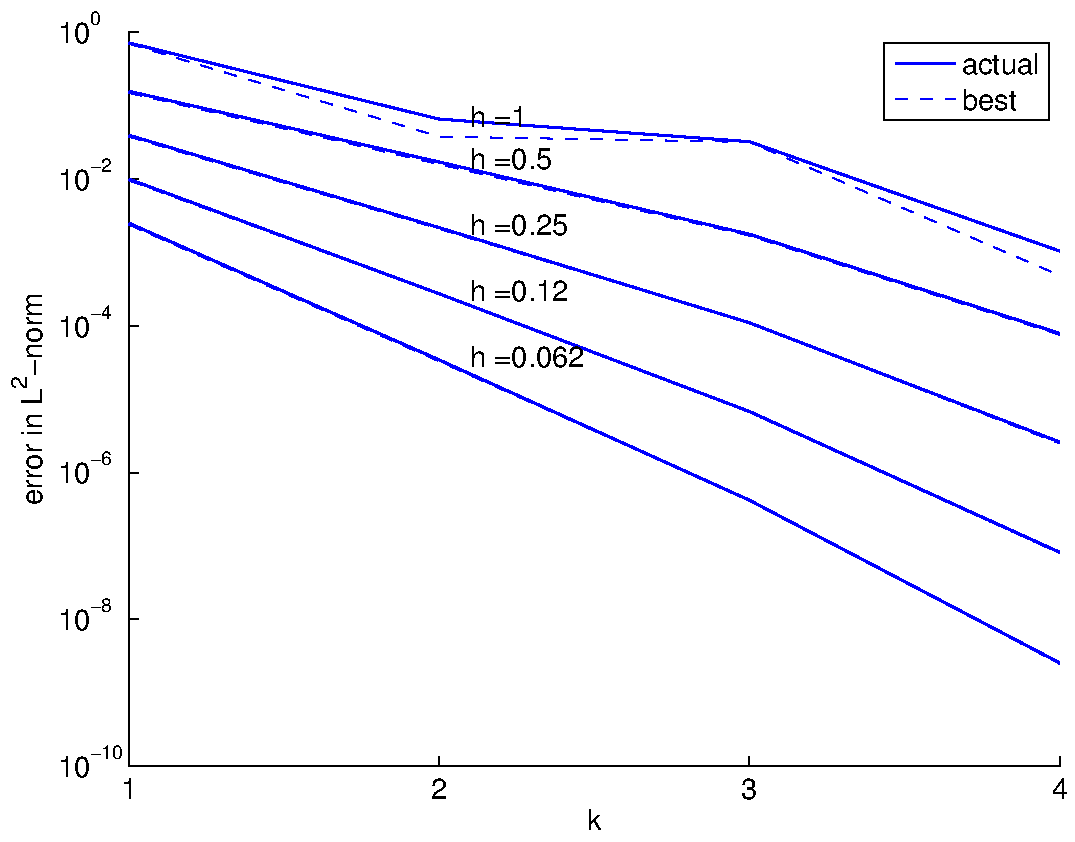
\includegraphics[scale=0.42]{./figures/u2_naive_p.pdf}
\label{fig:u2naive_p}
}
\subfigure[$p$]{
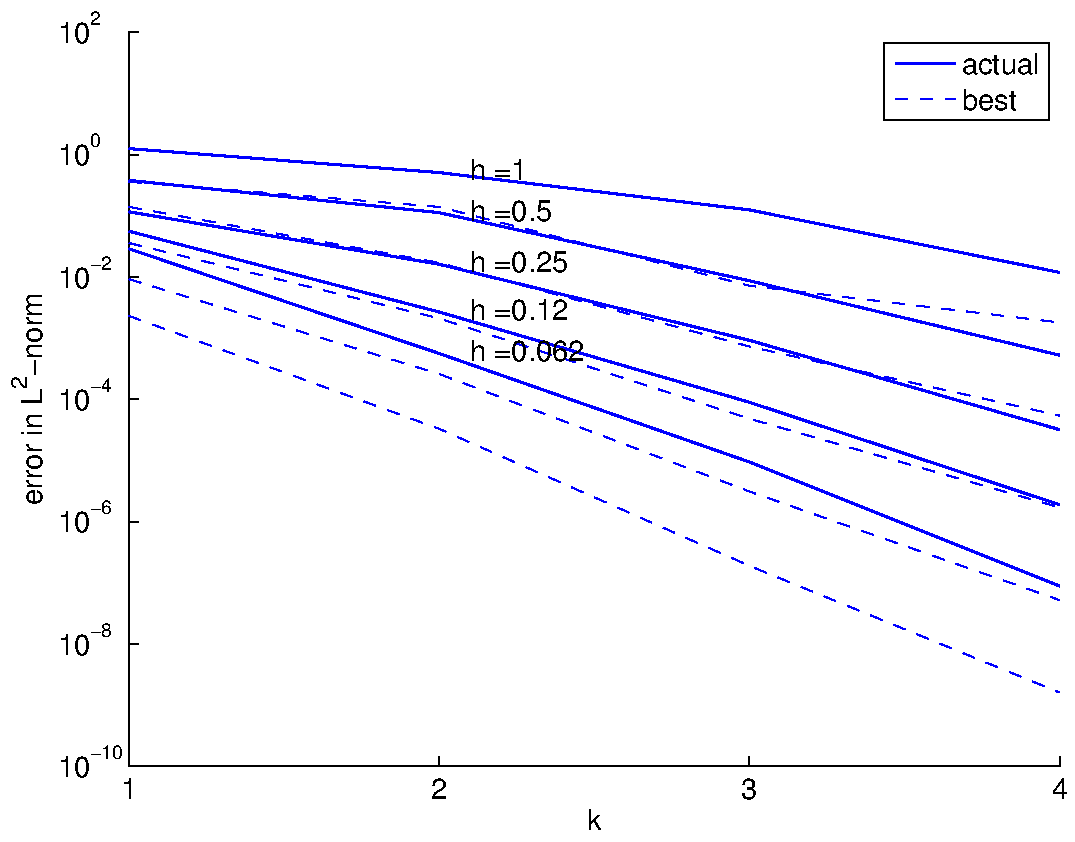
\includegraphics[scale=0.42]{./figures/pressure_naive_p.pdf}
\label{fig:pressurenaive_p}
}
\caption{p-convergence of $u_{1},u_{2}$ and $p$ when using the naive norm for the test space.  We observe exponential convergence for the finer meshes, and nearly match the $L^{2}$-projection of the exact solution for $u_{1}$ and $u_{2}$, but see significantly suboptimal solutions in $p$.
}
\label{fig:naive_p}
\end{figure}

\subsection{Lid-Driven Cavity Flow}
A classic test case for Stokes flow is the lid-driven cavity flow problem.  Consider a square cavity with an incompressible, viscous fluid, with a lid that moves at a constant rate.  The resulting flow will be vorticular; as sketched in Figure \ref{fig:cavity_flow_cartoon}, there will also be so-called \emph{Moffat eddies} at the corners; in fact, the exact solution  will have an infinite number of such eddies, visible at progressively finer scales \cite{Moffat}.  Note that the problem as described will have a discontinuity in the fluid velocity at the top corners, and hence its solution will not conform to the spaces we used in our analysis; for this reason, in our experiment we approximate the problem by introducing a thin ramp in the boundary conditions---we have chosen a ramp of width $\frac{1}{64}$.  This makes the boundary conditions continuous,\footnote{It is worth noting that these boundary conditions are not exactly representable by many of the coarser meshes used in our experiments.  We interpolate the boundary conditions in the discrete space.} so that the solution conforms to the spaces used in the analysis.
\begin{figure}[h!b!p!]
\centering
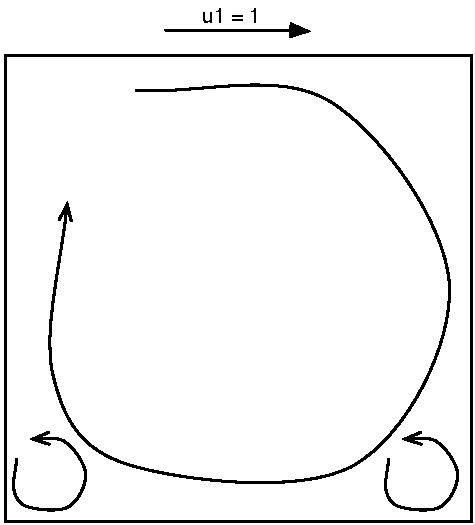
\includegraphics[scale=0.42]{./figures/cavity_flow_cartoon.pdf}
\caption{Sketch of lid-driven cavity flow.
}
\label{fig:cavity_flow_cartoon}
\end{figure}

As described in the introduction, DPG gives us a mechanism for measuring the residual error in the dual norm (the very error we seek to minimize) precisely, and we use this to drive adaptivity, by measuring the error $\norm{e_{K}}_{V}$ for each element $K$.  Both the method and our code allow refinements in $h$ or $p$ or in some combination of $h$ and $p$.  However, we do not yet have a general mechanism for deciding \emph{which} refinement to apply ($h$ or $p$), once we have decided that a given element should be refined.  We run two experiments, one with $h$-adaptivity and one using an ad hoc $hp$-adaptive strategy, described below.

Although it is not required by the code, we enforce \emph{1-irregularity} throughout---that is, before an element can be refined twice along an edge, its neighbor along that edge must be refined once.  In limited comparisons running the same experiments without enforcing 1-irregularity, this did not appear to make much practical difference.

\subsubsection{$h$-refinement strategy}
For $h$-refinements, our strategy is very simple:
\begin{enumerate}
\item Loop through the elements, determining the maximum element error $\norm{e_{K{\rm max}}}_{V}$.
\item Refine all elements with error at least 20\% of the maximum $\norm{e_{K{\rm max}}}_{V}$.
\end{enumerate}

Because the exact solution is unknown, we first solve on an overkill mesh and compare our adaptive solution at each step to the overkill solution.  In this experiment, we used quadratic field variables ($k=2$), a test space enrichment of 1 relative to the $H^{1}$ order (that is, $k_{\rm test} = k + 2 = 4$) for both the adaptive and overkill solutions.  The overkill mesh was $256 \times 256$ elements, with 5,576,706 dofs.

The initial mesh was a $2 \times 2$ square mesh; we ran seven $h$-adaptive refinements.  We stopped after seven steps to ensure that the resulting mesh was nowhere finer than the overkill solution.  At each step, we computed the Euclidean ($\ell_{2}$) norm of the $L^{2}$ norm of each of the seven field variables.  The final adaptive mesh has 124 elements and 11,202 dofs, and combined $L^{2}$ error of $4.4 \times 10^{-4}$ compared with the overkill mesh.  We also ran a few uniform refinements and computed the $L^{2}$ error for these compared with the overkill mesh, to show the comparative efficiency of the adaptive refinements.  The results are plotted in Figure \ref{fig:adaptive_cavity_flow_quadratic_vs_overkill}.
\begin{figure}[h!b!p!]
\centering
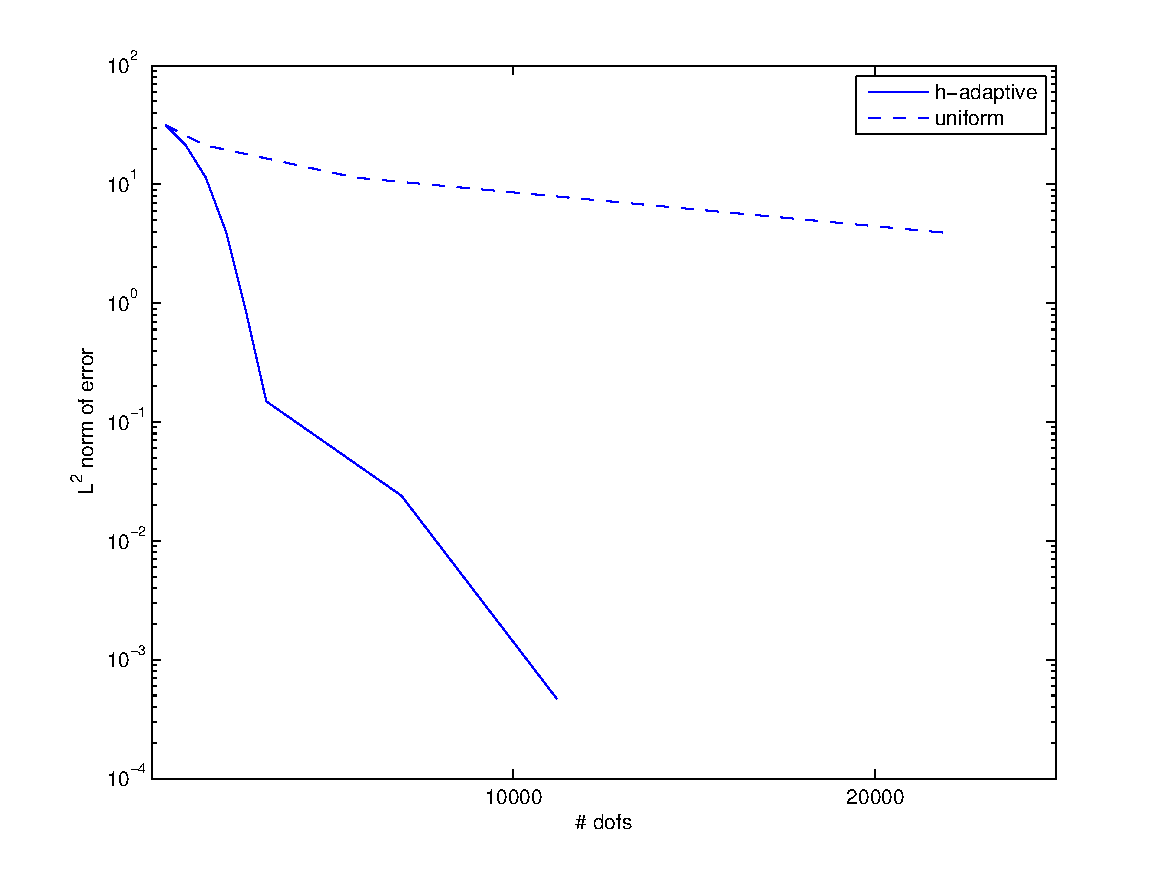
\includegraphics[scale=0.60]{./figures/adaptive_cavity_flow_quadratic_vs_overkill.pdf}
\caption{Euclidean norm of $L^{2}$ error in all field variables in $h$-adaptive mesh relative to an overkill mesh with $256 \times 256$ quadratic elements.  The Euclidean norm of all field variables in the exact solution is 6.73.
}
\label{fig:adaptive_cavity_flow_quadratic_vs_overkill}
\end{figure}

We also post-processed the results to solve for the stream function $\phi$, where $\Delta \phi = \NVRcurl \vect{u}$.  The contours of $\phi$ are the streamlines of the flow.  These are plotted for the quadratic adaptive mesh described above in Figure \ref{fig:streamlines_p2}; the first Moffat eddy can be seen clearly in the zoomed-in plot.  This quadratic mesh does not resolve the second Moffat eddy, but if we run 11 adaptive refinements on a cubic mesh, we can see it.  This is shown in Figure \ref{fig:streamlines_p3_r11}.

\begin{figure}[h!b!p!]
\centering
\subfigure[full cavity]{
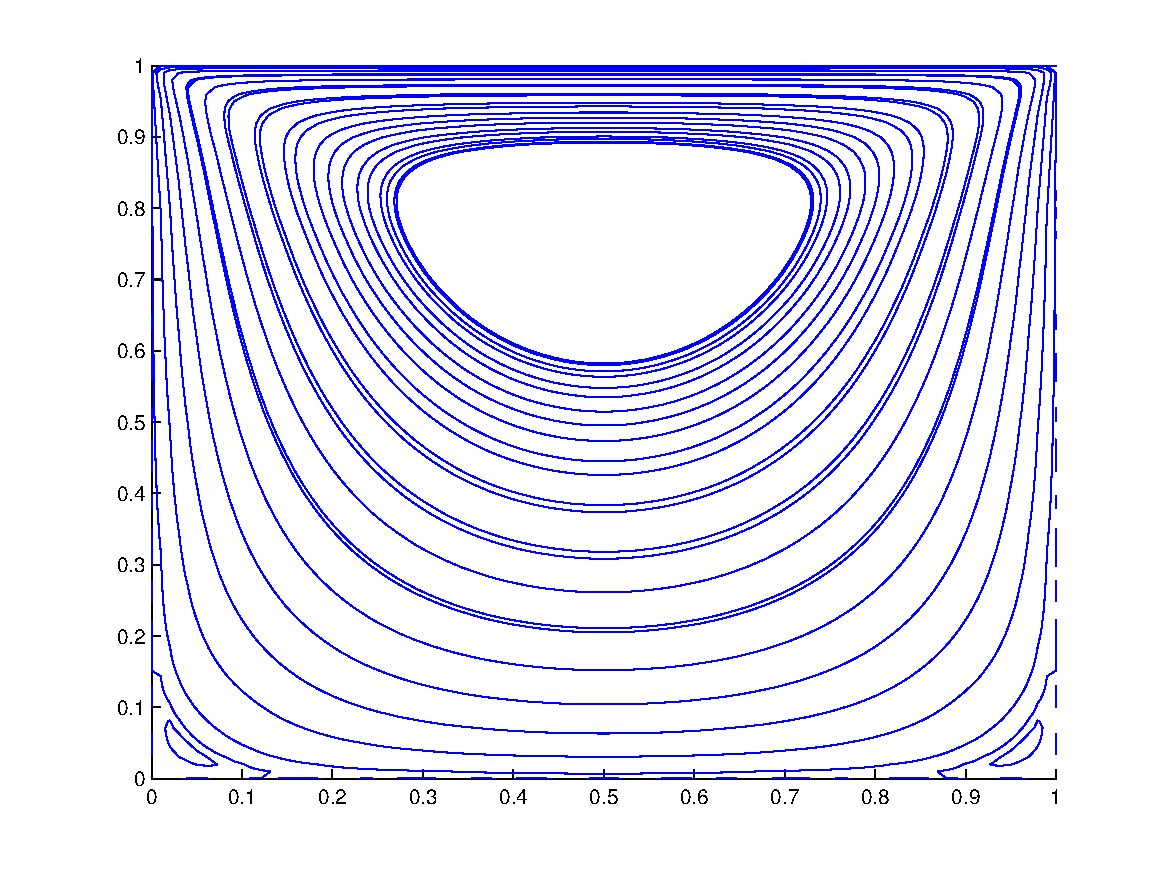
\includegraphics[scale=0.42]{./figures/streamlines_p2_r7.pdf}
\label{fig:streamlines_p2_r7}
}
\subfigure[lower-left corner]{
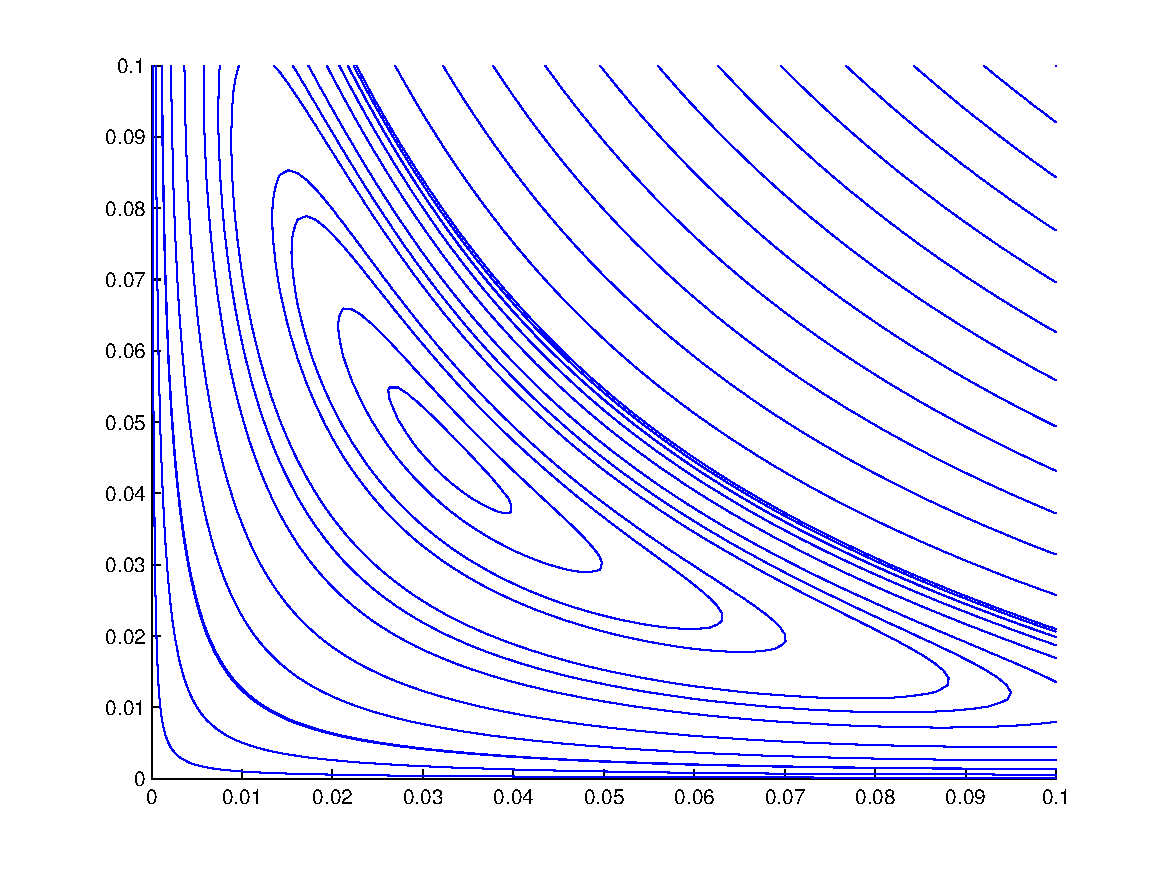
\includegraphics[scale=0.42]{./figures/streamlines_detail_p2_r7.pdf}
\label{fig:streamlines_detail_p2_r7}
}
\caption{Streamlines for the full cavity and for the lower-left corner, on a quadratic mesh after 7 adaptive refinements.  The lower-left corner shows the first Moffat eddy.  The final mesh has 124 elements and 11,202 dofs.}
\label{fig:streamlines_p2}
\end{figure}

\begin{figure}[h!b!p!]
\centering
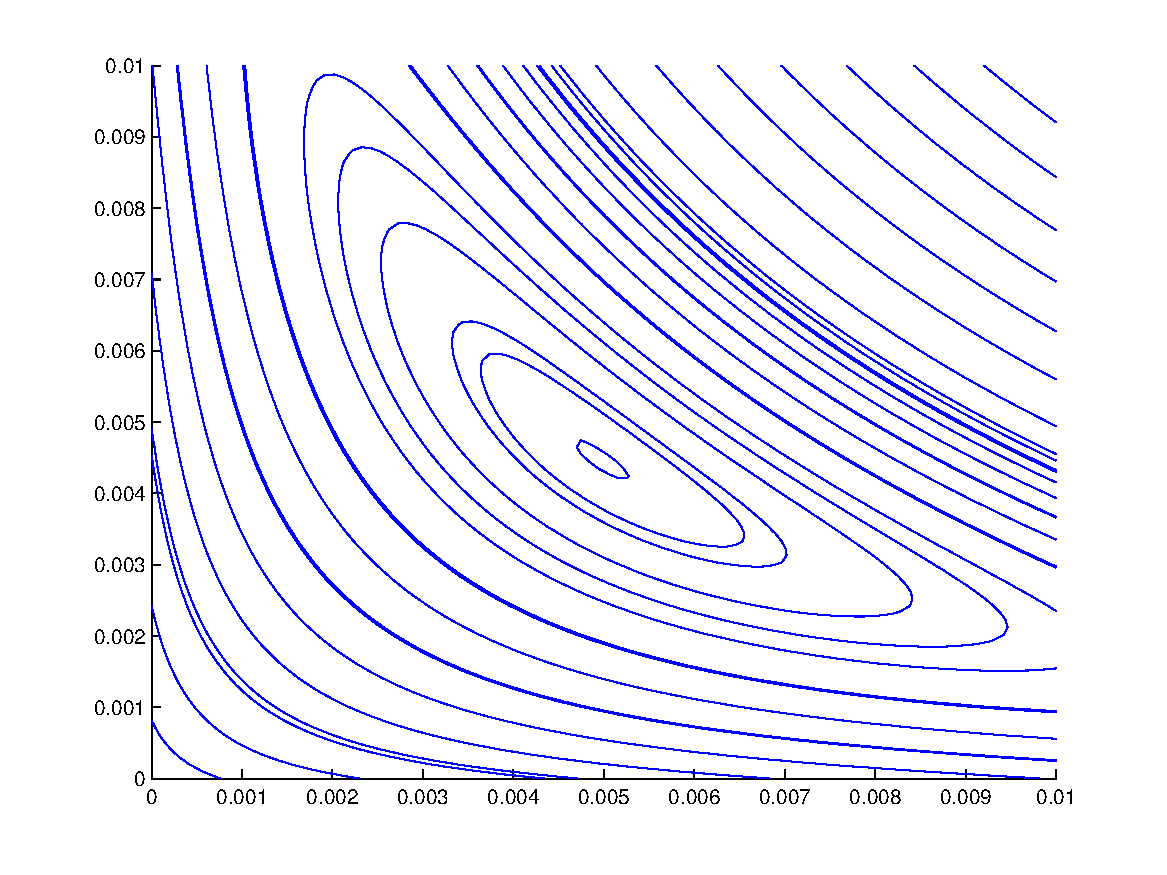
\includegraphics[scale=0.42]{./figures/streamlines_minute_detail_p3_r11.pdf}
\caption{Streamlines for the lower-left corner on a cubic mesh after 11 adaptive refinements: the second Moffat eddy.  The final mesh has 298 elements and 44,206 dofs.}
\label{fig:streamlines_p3_r11}
\end{figure}

\subsubsection{Ad hoc $hp$-refinement strategy}
For the $hp$ experiment, we adopt a similar strategy; this time, our overkill mesh contains $64 \times 64$ quintic elements, and our initial mesh has $2 \times 2$ linear elements.  We know {\it a priori} that we should refine in $h$ at the top corners---if only to fully resolve the boundary condition.  The strategy is again:
\begin{enumerate}
\item Loop through the elements, determining the maximum element error $\norm{e_{K{\rm max}}}_{V}$.
\item Refine all elements with error at least 20\% of the maximum $\norm{e_{K{\rm max}}}_{V}$.
\end{enumerate}
However, this time we must decide whether to refine in $h$ or $p$.  The basic constraints we would like to follow are:
\begin{itemize}
\item the adaptive mesh must be nowhere finer than the overkill mesh (in $h$ or $p$), and
\item prefer $h$-refinements at all corners (top and bottom).
\end{itemize}
So, once the corner elements are as small as the overkill mesh, then they refine in $p$, and all other elements refine in $p$ until they are quintic, after which they may refine in $h$.

The primary purpose of this experiment is to demonstrate that the method allows arbitrary meshes of arbitrary, variable polynomial order.  The strategy described above clearly depends on \emph{a priori} knowledge of the particular problem we are solving; we have yet to determine a good general strategy for deciding between $h$- and $p$-refinements.

We ran 9 refinement steps.  The final mesh has 46 elements and 5,986 dofs, compared with 1,223,682 dofs in the overkill mesh.  The $L^{2}$ error of the adaptive solution compared with the overkill is $8.0 \times 10^{-4}$.  As in the previous experiment, we also tried running a few uniform $h$-refinements on the same initial mesh, as a baseline for comparison.  The results are plotted in Figure \ref{fig:hp_adaptive_cavity_flow_vs_overkill}; the mesh can be seen in Figure \ref{fig:cavityFlowPolyOrder}.

\begin{figure}[h!b!p!]
\centering
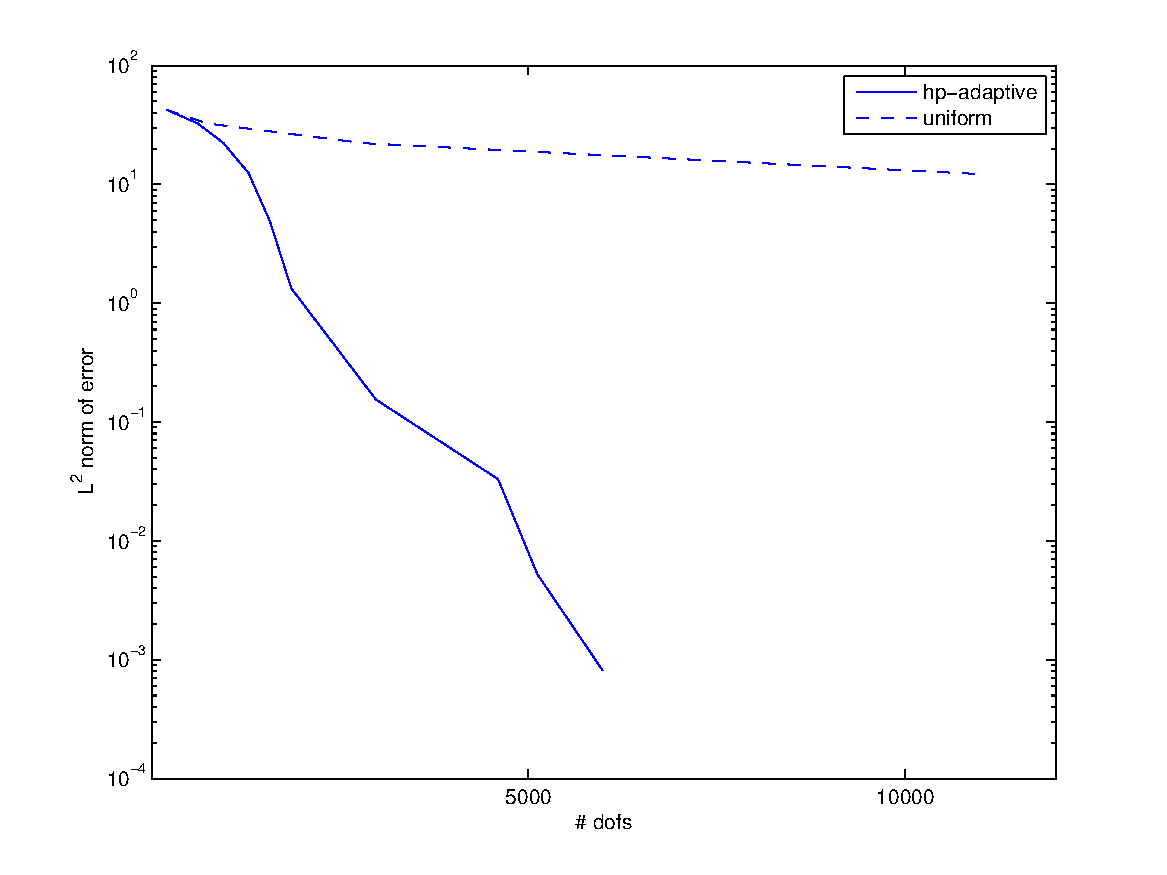
\includegraphics[scale=0.60]{./figures/hp_adaptive_cavity_flow_vs_overkill.pdf}
\caption{Euclidean norm of $L^{2}$ error in all field variables in (ad hoc) $hp$-adaptive mesh relative to an overkill mesh with $64 \times 64$ quintic elements.  The Euclidean norm of all field variables in the exact solution is 6.73; the final mesh has 46 elements and 5,986 dofs.
}
\label{fig:hp_adaptive_cavity_flow_vs_overkill}
\end{figure}

\begin{figure}[h!b!p!]
\centering
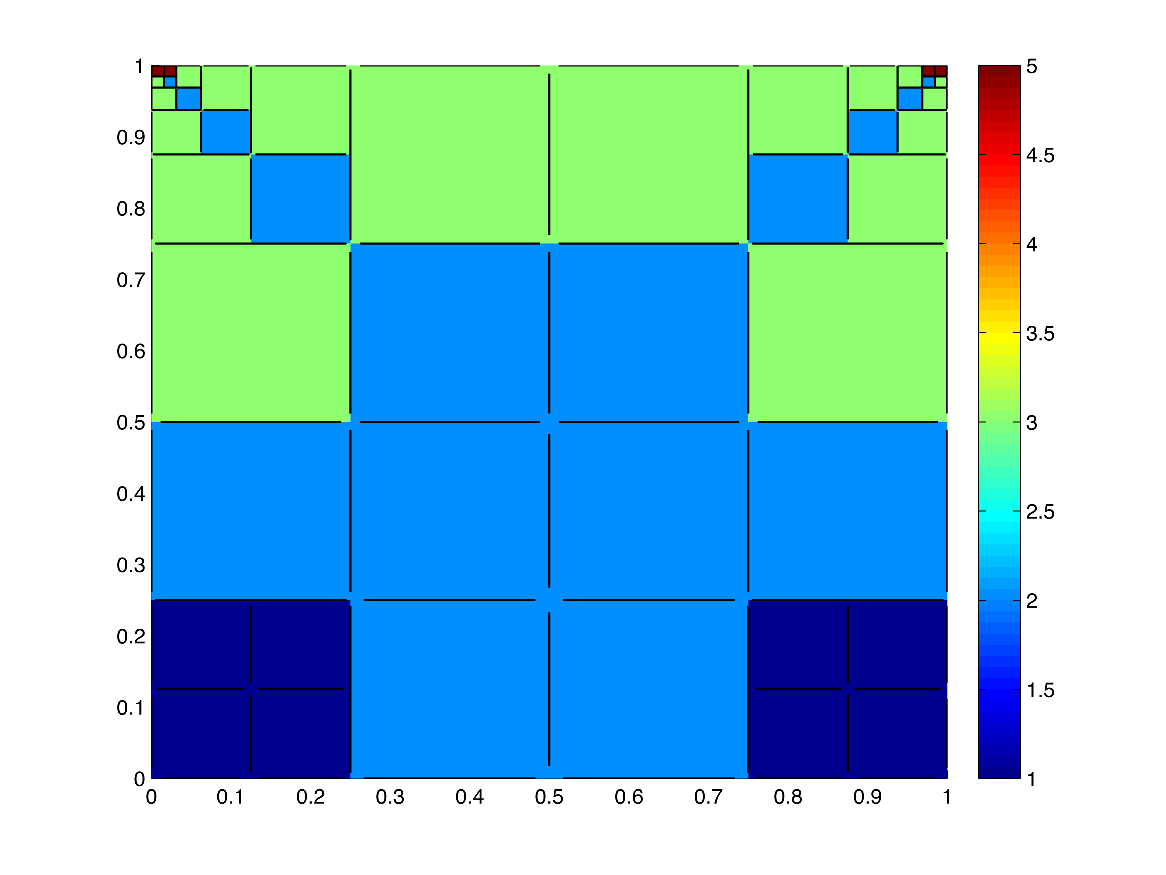
\includegraphics[scale=0.60]{./figures/cavityFlowPolyOrder.pdf}
\caption{Adaptive mesh for ad hoc $hp$-adaptivity strategy after 9 refinement steps.  The scale represents the polynomial order of the $L^{2}$ variables in the solution.  The final mesh has 46 elements and 5,986 dofs.
}
\label{fig:cavityFlowPolyOrder}
\end{figure}